\documentclass{article}

\usepackage[portuguese]{babel}
\usepackage[utf8]{inputenc}
\usepackage{graphicx}
\usepackage{eso-pic}
\usepackage{float}

\AddToShipoutPictureBG{\AtPageUpperLeft{\raisebox{-\height}{
\includegraphics[width=2in]{logo}}}}

\begin{document}

\title{Ambientes Virtuais de Execução \\ Benchmarking ao Garbage Collector da VM LUA}
\author{Daniel Dias Gonçalves \\ Nº 68126 \\ daniel.dias.g@gmail.com}
\maketitle

\begin{abstract}
Lua é uma linguagem de programação que tem como objectivo a extensão de aplicações. Com este relatório pretende-se realizar uma avaliação à gestão de memória da máquina virtual Lua, discutindo os resultados obtidos com base em \emph{micro-brenchmarkings} realizados.
\end{abstract}

%
\section{Introdução}
\label{sec:intro}
%
Uma das grandes preocupações a ter ao desenvolver uma máquina virtual é como é gerida a memória. Cada vez mais as máquinas virtuais de linguagens de alto nível, como Lua VM, usam gestão de memória automática (através do \emph{Garbage Collector}) sendo que para o programador tem as seguintes vantagens:
\begin{itemize}
\item Não existe a preocupação de alocar memória para novos objectos.
\item Não é necessário fazer \emph{free} aos objetos que não são mais necessários.
\end{itemize}

Actualmente existem vários algoritmos de \emph{garbage collecting} sendo que não existe um que seja considerado o melhor para todos os casos. Alguns desses algoritmos são: (1) \emph{Mark and Sweep} (2) \emph{Compacting} (3) \emph{Copying} (4) Incrementais. Ao longo deste trabalho estamos interessados no algoritmo \emph{Mark and Sweep} incremental.

Lua é uma linguagem de programação desenvolvida para a extensão de programas, existindo uma grande procura por programas customizáveis.
Existem vários tipos de linguagens de extensão, tais como (1) \emph{configuration languages} (2) \emph{scripting languages} (3) \emph{macro languages} (4) \emph{embedded languages}.
O propósito de Lua é ser uma \emph{embedded language}, ou seja extender aplicações com funções definidas pelo utilizador baseadas nas primitivas fornecidas pelas aplicações.

Este trabalho tem como objectivo analisar a implementação do algoritmo de \emph{Garbage Collection} da máquina virtual Lua. Para isso será apresentado e explicado, com referências ao código, a sua implementação actual. De seguida serão apresentados os resultados obtidos na realização de \emph{micro-brenchmarking} e por fim discutido os resultados obtidos.

%
\section{Tecnologia de Virtualização e Mecânismos Internos Estudados}
\label{sec:estudo}
%
Esta secção está organizada da seguinte forma - na secção~\ref{subsec:basico} será feito uma breve apresentação da máquina virtual e linguagem Lua; e por fim na secção~\ref{subsec:gc} será explicada a implementação do \emph{Garbage Collector} da máquina virtual LUA. 

%
\subsection{Linguagem Lua e Máquina Virtual}
\label{subsec:basico}
%

\subsubsection{Tipos de Dados}
Lua não exige tipos nas variáveis, pois é capaz de escolher que tipo usar dinamicamente.
Deste modo os valores têm o seu próprio tipo:
\begin{description}
\item[nil.] Valor da variável antes da primeira atribuição.
\item[number.] Representa números reais.
\item[string.] Cadeia de caracteres.
\item[function.] Funções definidas pelo utilizador.
\item[Cfunction.] Funções fornecidas pela aplicação a ser extendida.
\item[userdata.] Apontadores para dados arbitrários em C.
\item[table.] Arrays associativos, ou seja podem ser indexados por números ou strings.
\item[threads.] É usado para representar corotinas.
\item[booleans.] Representa true ou false.
\end{description}

Os valores são implementados numa estrutura com dois campos: um tipo e uma \emph{union} que contêm o seu valor actual.
Os números são guardados directamente dentro da união. As \emph{strings} são mantidas num array, sendo que o valor \emph{strings} contem apontadores para esse array. Valores do tipo \emph{Cfunction} contêm o apontador para a função C e valores do tipo \emph{userdate} contêm apontadores para os dados. \emph{Tables} são implementadas como hash-tables.

A especificação das estruturas pode ser encontrada no ficheiro 'lobject.h'.

\subsubsection{Máquina Virtual}
Programas para a máquina virtual são sequências de intruções, chamados \emph{bytecodes}, sendo que a execução desses programas é feita através da interpretação dos mesmos.

Podemos encontrar a implementação do ciclo principal da máquina virtual no ficheiro 'lvm.c' na seguinte função:
\begin{verbatim}
#define RA(i)   (base+GETARG_A(i))
#define RB(i)   check_exp(getBMode(GET_OPCODE(i)) 
                     == OpArgR, base+GETARG_B(i))

...

1.  void luaV_execute (lua_State *L) {
2.  ...
3.  for (;;) {
4.      Instruction i = *(ci->u.l.savedpc++);
5.  ...
6.  ra = RA(i);
7.  ...
8.  vmdispatch (GET_OPCODE(i)) {
9.  vmcase(OP_MOVE,
10.          setobjs2s(L, ra, RB(i));
11.       )
12. ...
\end{verbatim}

Como podemos observar dentro do ciclo o primeiro passo a ser realizado é carregar a instrução relativamente a um PC (program counter) guardado, linha 4.
Na linha 8 é extraido da intrução o opcode correspondente. Uma vez encontrado o opcode, é usado um grande switch para encontrar a operação a executar. No código apresentado podemos ver na linha 9 o caso de ser a operação MOVE.

%
\subsection{Garbage Collector}
\label{subsec:gc}
%
O \emph{garbage collector}  máquina virtual LUA 5.2 por definição usa o algoritmo \emph{Incremental Mark and Sweep}, existindo a possíbilidade de usar o algoritmo \emph{Generational}.
Neste trabalho estamos interessados em analisar o algoritmo que está seleccionado por definição, uma vez ser o mais estável e usado.
Basicamente a implementação do \emph{Garbage Collector} é constituida por duas fases:
\begin{itemize}
\item Fase \emph{mark}. Nesta fase o GC começa nas referências do conjunto root, e iterativamente marca todos os objectos a que consegue chegar.
\item Fase \emph{sweep}. Nesta fase todos os objectos a que não foi possível chegar são libertados.
\end{itemize}

Para não existir grandes paragens durante a execução, o algoritmo de \emph{garbage collection} é executado por diversos passos (ou seja é Incremental).

Neste algoritmo cada objecto pode ter uma das seguintes cores:
\begin{description}
\item[Branco.] O objecto ainda não foi marcado.
\item[Cinzento.] O objecto foi marcado, mas as suas referências podem ainda não ter sido.
\item[Preto.] O objecto e todas as suas referências foram marcadas.
\end{description}

Todo o trabalho de marcar e detetar a cor de um determinado objecto é feito no campo chamado 'marked' com operações a bits.
No código podemos encontrar a seguinte definição:
\begin{verbatim}
/* Layout for bit use in `marked' field: */
#define WHITE0BIT       0  /* object is white (type 0) */
#define WHITE1BIT       1  /* object is white (type 1) */
#define BLACKBIT        2  /* object is black */
...
#define WHITEBITS       bit2mask(WHITE0BIT, WHITE1BIT)
#define iswhite(x)      testbits((x)->gch.marked, WHITEBITS)
#define isblack(x)      testbit((x)->gch.marked, BLACKBIT)
#define isgray(x)  /* neither white nor black */  \
        (!testbits((x)->gch.marked, WHITEBITS | bitmask(BLACKBIT)))
\end{verbatim}
Sendo que a macro testbits e testbit verificam o valor dos bits correspondentes.
Podemos facilmente ver que os bits 0 e 1 indicam se o objecto é branco, o bit 2 indica se o objecto é preto e caso nenhum destes estaja marcado é considerado cinzento.

\begin{figure}[h!]
    \centering
    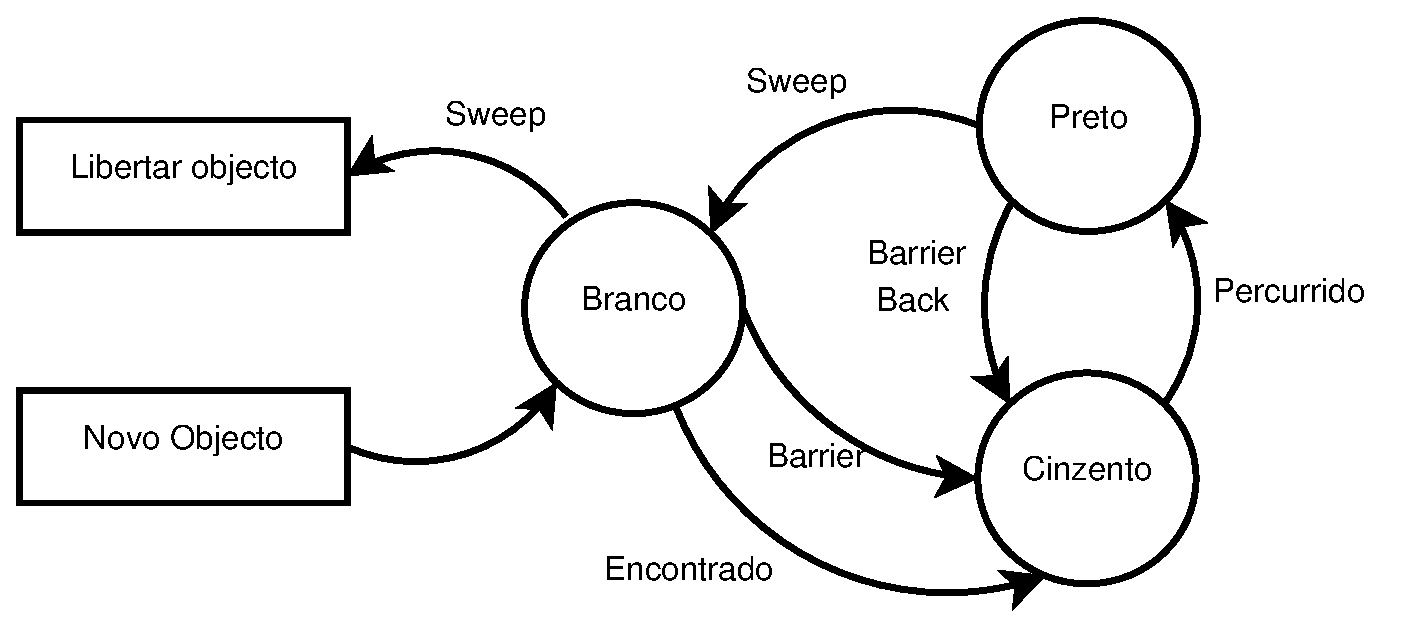
\includegraphics[width=0.8\textwidth]{GC-algoritm.eps}
    \caption{Mark and Sweep Incremental}
    \label{fig:marksweep}
\end{figure}

Na figura~\ref{fig:marksweep} são apresentados os diversos passos, sendo que a explicação da mesma encontra-se de seguida.

Inicialmente é feita uma pesquisa do conjunto root (o conjunto onde começa a pesquisa) pela pilha e registos do programa, sendo que todos os novos objectos são brancos.
A fase de \emph{mark} começa então na pesquisa do conjunto root, marcando todos a que consegue chegar, ou seja muda a cor desses objectos de branco para cinzento.
Cada um dos objectos marcados como cinzento é percorrido de forma a marcar todos os objectos referênciados por ele. Por fim esse objecto é colocado como preto. 

Na fase de \emph{sweep} todos os objectos que têm a cor branca são libertados e os objectos de cor preto são marcados de volta para a cor branca.

Devido a este algoritmo ser incremental, ou seja é executado em pequenos passos, o código da \emph{garbage collector} e do programa são executados intercaladamente.
Desta forma é possível que o programa altere uma referência de um objecto preto e que passe a apontar para um branco, causando o problema de que este objecto pode nunca ser visitado e ser libertado da memória.
Para resolver este problema existe a seguinte invariante:
\begin{itemize}
\item Um objecto preto nunca pode ter uma referência para um objecto branco.
\end{itemize}

Como na fase de sweep esta invariante pode não ser obedecida, foi  criada a seguinte macro que se encontra definida no ficheiro 'lgc.h' de forma a saber quando aplicá-la (devido a não estarmos a analisar o algoritmo \emph{Generational} só nos interessa a segunda parte do 'ou'):
\begin{verbatim}
#define keepinvariant(g)        (isgenerational(g) ||
                                   g->gcstate <= GCSatomic)
\end{verbatim}

Para compreensão da macro apresentada é importante referir os vários estados do \emph{garbage collector} também definidos nesse header:
\begin{verbatim}
#define GCSpropagate    0
#define GCSatomic       1
#define GCSsweepstring  2
#define GCSsweepudata   3
#define GCSsweep        4
#define GCSpause        5
\end{verbatim}

Em cada ciclo o algoritmo passa por um destes estados, através de uma função definida no ficheiro 'lgc.c' usando um \emph{switch}:
\begin{verbatim}
static lu_mem singlestep (lua_State *L)
\end{verbatim}

De seguida é apresentado a definição de cada um dos estados pela ordem que são executados:
\begin{description}
\item[GCSpause.] Neste estado todos os objectos devem ser marcados com a cor branca do tipo seleccionado a ser usado. O 'lua\_State', a tabela global, os registos e as metatables são marcados como cinzentos e adicionados à lista de cinzentos.
\item[GCSpropagate.] Cada objecto na lista de cinzentos é removido e marcado como preto, sendo que todos os objectos brancos que este referencia são marcados como cinzentos e adicionados à lista de cinzentos. Uma vez que a lista cinzenta esteja vazia todos os brancos do tipo definido como actual são mudados para o outro tipo e todos os objectos de cor branca de tipo diferente são considerados objectos a serem libertos.
\item[GCSsweepstring.] A cor de cada string é verificada, sendo que se a cor for igual ao antigo tipo da cor branca essa string pode ser libertada.
\item[GCSsweepudata.] Da mesma forma que o estado anterior vai iterar pelos userdata, verificando a cor dos mesmos, sendo que aos objectos não referenciados é executado o seu metamethod.
\item[GCSsweep.] A cor de cada objecto na lista global root é verificado e como os dois estados anteriores os objectos que com o tipo antigo da cor branca podem ser removidos.
\end{description}

Quando a invariante referida anteriormente não se verifica, existem duas soluções:
\begin{itemize}
\item Colocar o objecto preto de volta para cinzento (barrier back), ou
\item Marcar o objecto branco para cinzento (barrier).
\end{itemize}

Como foi dito anteriormente o \emph{garbage collector} é executado por pequenos passos. 
Existem dois números, que podem ser mudados pelo utilizador, de modo a controlar os seus ciclos:
\begin{description}
\item[Garbage collector pause.] É usado para controlar quanto tempo o \emph{garbage collector} tem de esperar até ser chamado outra vez. Valores muito baixos significam que vai existir um grande desperdicio de  tempo a executar o algoritmo, em contra partida valores muito altos pode levar a que o programa use demasiada memória.
\item[Garbage collector step multiplier.] Controla a velocidade a que é executado o garbage collector, ou seja um valor alto significa que cada passo vai ser maior.
\end{description}

Existem várias funções disponibilizadas para que, quem está a desenvolver um programa, consiga ter algum controlo.
Podemos ver no ficheiro 'lbaselib.c' as várias funções que podem ser chamadas:
\begin{verbatim}
static int luaB_collectgarbage (lua_State *L) {
  static const char *const opts[] = {"stop", "restart", "collect",
    "count", "step", "setpause", "setstepmul",
    "setmajorinc", "isrunning", "generational", "incremental", NULL};
  static const int optsnum[] = {LUA_GCSTOP, LUA_GCRESTART, LUA_GCCOLLECT,
    LUA_GCCOUNT, LUA_GCSTEP, LUA_GCSETPAUSE, LUA_GCSETSTEPMUL,
    LUA_GCSETMAJORINC, LUA_GCISRUNNING, LUA_GCGEN, LUA_GCINC};
\end{verbatim}

De seguida é apresentado qual o objectivo de algumas dessas funções (as que considero mais importantes).
\begin{description}
\item[collectgarbage("collect").] Executa um ciclo completo.
\item[collectgarbage("count").] Retorna a quantidade de memória actualmente usada pelo programa.
\item[collectgarbage("restart").] No caso de ter sido parado o algoritmo, reinicia-o.
\item[collectgarbage("setpause").] Atribui o valor \emph{garbage collector pause} anteriormente falado.
\item[collectgarbage("setstepmul").] Atribui o valor \emph{garbage collector step multiplier} anteriormente falado.
\item[collectgarbage("step").] Executa um passo do algoritmo.
\item[collectgarbage("stop").] Pára o \emph{garbage collector}.
\end{description}

A implementação de cada uma destas funções pode ser encontrada no ficheiro 'lapi.c' na função,
\begin{verbatim}
LUA_API int lua_gc (lua_State *L, int what, int data)
\end{verbatim}
, que consiste num \emph{switch} para cada uma das opções.

%
\section{Avaliação do Garbage Collector}
\label{sec:aval}
%
Nesta secção é apresentado como vai ser analisado o desempenho do \emph{garbage collector} desenvolvendo micro-benchmarkings. Todos os testes apresentados neste relatório foram executados num sistema com um processador dual-core 64bits, com 4GB de memória RAM com o sistema operativo ArchLinux.

Segundo a secção anterior, podemos verificar que parte do tempo em que um determinado programa está a executar é ocupado pelo algoritmo de \emph{garbage collecting}. Deste modo numa primeira análise é de interesse saber qual o seu custo em termos do tempo.
Esta análise inicialmente será feita sobre um programa que só tem memória a ser libertada no final, ou seja todos os objectos são de longa duração. Depois será então analisado o tempo num programa que tenha objectos de curta e longa duração. O objectivo da existência destas duas análises é conseguir comparar o custo de percorrer a primeira fase, \emph{mark}, e a segunda fase, \emph{sweep}. Foi utilizado os programas em anexo A1 e A2 respectivamente.

Outro aspecto interessante é observar se o GC faz o que deve fazer, ou seja libertar memória. Para isso foram criados vários objectos, e removidas referências para alguns deles. Depois o GC foi obrigado a executar de modo a conseguir obter dados da quantidade de memória ao longo da execução do programa. Este código pode ser observado no anexo B.

Com base no código anterior pretende-se obter informação do tempo que o GC demora a colectar determinada quantidade de memória. O código adaptado do anterior encontra-se no anexo C.

No anexo D1 e D2 podemos encontrar o teste para medir o tempo de alocação de objectos. Foi medido em duas situações, onde diferenças são mais provaveis de existir:
\begin{itemize}
\item Tempo de alocação de objectos quando já foram removidos outros anteriores pelo GC e;
\item Tempo de alocação de objectos sem que tenham sido removidos outros pelo GC.
\end{itemize}

%
\section{Resultados da Avaliação}
\label{sec:res}
%
Nesta secção pretende-se apresentar os resultados das avaliações discutidas na secção~\ref{sec:aval}.

Como discutido anteriormente parte do tempo da execução do programa é ocupado pelo algoritmo de \emph{garbage collecting}.
Foi portanto analisado a execução de um programa que só contem objectos de longa duração com o GC activo e desactivo. O resultado obtido pode ser visualizado na figura~\ref{graph:graph1}. 
\begin{figure}[h!]
  \begin{center}
    \input{table1.tex}
    \caption{Eixo X: número de objecto em milhares. Eixo Y: duração da execução em segundos. Comparação entre o tempo de execução e número de objectos criados (longa duração), com  e sem o  GC activo}
    \label{graph:graph1}
  \end{center}
\end{figure}

Numa primeira análise podemos afirmar que como os objectos são todos de longa duração, o GC executa na maioria do tempo a primeira fase, \emph{Mark}.
Na figura podemos observar que não existe um impacto significativo, pois o tempo de execução das duas linhas são identicas para qualquer número de objectos criados.

Alguns dos picos que aparecem nas análises são devido às condições do ambiente de teste não serem as melhores.

Como a maioria dos programas não tem só objectos de longa duração, e de modo a comparar as duas fases do algoritmo, é mostrado na figura~\ref{graph:graph2} a mesma avaliação incluindo objectos de curta duração.


\begin{figure}[h!]
  \begin{center}
    % GNUPLOT: LaTeX picture with Postscript
\begingroup
  \makeatletter
  \providecommand\color[2][]{%
    \GenericError{(gnuplot) \space\space\space\@spaces}{%
      Package color not loaded in conjunction with
      terminal option `colourtext'%
    }{See the gnuplot documentation for explanation.%
    }{Either use 'blacktext' in gnuplot or load the package
      color.sty in LaTeX.}%
    \renewcommand\color[2][]{}%
  }%
  \providecommand\includegraphics[2][]{%
    \GenericError{(gnuplot) \space\space\space\@spaces}{%
      Package graphicx or graphics not loaded%
    }{See the gnuplot documentation for explanation.%
    }{The gnuplot epslatex terminal needs graphicx.sty or graphics.sty.}%
    \renewcommand\includegraphics[2][]{}%
  }%
  \providecommand\rotatebox[2]{#2}%
  \@ifundefined{ifGPcolor}{%
    \newif\ifGPcolor
    \GPcolorfalse
  }{}%
  \@ifundefined{ifGPblacktext}{%
    \newif\ifGPblacktext
    \GPblacktexttrue
  }{}%
  % define a \g@addto@macro without @ in the name:
  \let\gplgaddtomacro\g@addto@macro
  % define empty templates for all commands taking text:
  \gdef\gplbacktext{}%
  \gdef\gplfronttext{}%
  \makeatother
  \ifGPblacktext
    % no textcolor at all
    \def\colorrgb#1{}%
    \def\colorgray#1{}%
  \else
    % gray or color?
    \ifGPcolor
      \def\colorrgb#1{\color[rgb]{#1}}%
      \def\colorgray#1{\color[gray]{#1}}%
      \expandafter\def\csname LTw\endcsname{\color{white}}%
      \expandafter\def\csname LTb\endcsname{\color{black}}%
      \expandafter\def\csname LTa\endcsname{\color{black}}%
      \expandafter\def\csname LT0\endcsname{\color[rgb]{1,0,0}}%
      \expandafter\def\csname LT1\endcsname{\color[rgb]{0,1,0}}%
      \expandafter\def\csname LT2\endcsname{\color[rgb]{0,0,1}}%
      \expandafter\def\csname LT3\endcsname{\color[rgb]{1,0,1}}%
      \expandafter\def\csname LT4\endcsname{\color[rgb]{0,1,1}}%
      \expandafter\def\csname LT5\endcsname{\color[rgb]{1,1,0}}%
      \expandafter\def\csname LT6\endcsname{\color[rgb]{0,0,0}}%
      \expandafter\def\csname LT7\endcsname{\color[rgb]{1,0.3,0}}%
      \expandafter\def\csname LT8\endcsname{\color[rgb]{0.5,0.5,0.5}}%
    \else
      % gray
      \def\colorrgb#1{\color{black}}%
      \def\colorgray#1{\color[gray]{#1}}%
      \expandafter\def\csname LTw\endcsname{\color{white}}%
      \expandafter\def\csname LTb\endcsname{\color{black}}%
      \expandafter\def\csname LTa\endcsname{\color{black}}%
      \expandafter\def\csname LT0\endcsname{\color{black}}%
      \expandafter\def\csname LT1\endcsname{\color{black}}%
      \expandafter\def\csname LT2\endcsname{\color{black}}%
      \expandafter\def\csname LT3\endcsname{\color{black}}%
      \expandafter\def\csname LT4\endcsname{\color{black}}%
      \expandafter\def\csname LT5\endcsname{\color{black}}%
      \expandafter\def\csname LT6\endcsname{\color{black}}%
      \expandafter\def\csname LT7\endcsname{\color{black}}%
      \expandafter\def\csname LT8\endcsname{\color{black}}%
    \fi
  \fi
  \setlength{\unitlength}{0.0500bp}%
  \begin{picture}(7200.00,5040.00)%
    \gplgaddtomacro\gplbacktext{%
      \csname LTb\endcsname%
      \put(594,440){\makebox(0,0)[r]{\strut{} 0}}%
      \put(594,874){\makebox(0,0)[r]{\strut{} 2}}%
      \put(594,1307){\makebox(0,0)[r]{\strut{} 4}}%
      \put(594,1741){\makebox(0,0)[r]{\strut{} 6}}%
      \put(594,2174){\makebox(0,0)[r]{\strut{} 8}}%
      \put(594,2608){\makebox(0,0)[r]{\strut{} 10}}%
      \put(594,3041){\makebox(0,0)[r]{\strut{} 12}}%
      \put(594,3475){\makebox(0,0)[r]{\strut{} 14}}%
      \put(594,3908){\makebox(0,0)[r]{\strut{} 16}}%
      \put(594,4342){\makebox(0,0)[r]{\strut{} 18}}%
      \put(594,4775){\makebox(0,0)[r]{\strut{} 20}}%
      \put(726,220){\makebox(0,0){\strut{} 0}}%
      \put(1594,220){\makebox(0,0){\strut{} 10000}}%
      \put(2462,220){\makebox(0,0){\strut{} 20000}}%
      \put(3330,220){\makebox(0,0){\strut{} 30000}}%
      \put(4199,220){\makebox(0,0){\strut{} 40000}}%
      \put(5067,220){\makebox(0,0){\strut{} 50000}}%
      \put(5935,220){\makebox(0,0){\strut{} 60000}}%
      \put(6803,220){\makebox(0,0){\strut{} 70000}}%
    }%
    \gplgaddtomacro\gplfronttext{%
      \csname LTb\endcsname%
      \put(5816,4602){\makebox(0,0)[r]{\strut{}"table2.dat" using 1:2}}%
      \csname LTb\endcsname%
      \put(5816,4382){\makebox(0,0)[r]{\strut{}"table2.dat" using 1:3}}%
    }%
    \gplbacktext
    \put(0,0){\includegraphics{table2}}%
    \gplfronttext
  \end{picture}%
\endgroup

    \caption{Eixo X: número de objecto em milhares. Eixo Y: duração da execução em segundos. Comparação entre o tempo de execução e número de objectos criados (curta e longa duração), com  e sem o  GC activo}
    \label{graph:graph2}
  \end{center}
\end{figure}

No caso da figura~\ref{graph:graph2} o GC já tem tarefas a realizar na segunda fase, \emph{Sweep}, pois existem objectos de curta duração.
Conseguimos observar que à medida que são criados mais objectos e libertados mais objectos o tempo de execução usando GC aumenta em relação à não utilização do mesmo.

Existe portanto um \emph{tradeoff}, pois é abdicado tempo para que a gestão de memória seja automática. No entanto visto não ser um aumento muito acentuado, na maioria das situações torna-se vantajoso.

Na figura~\ref{graph:graph3} podemos observar memória usada por um programa a ser liberta após ser executado o GC. Neste caso temos a representação da memória usada em bytes (eixo Y) ao longo do tempo de execução do programa em segundos (eixoX). No topo de cada pico é quando o algoritmo é executado, libertando todos os objectos que não são referênciados.
Com esta análise conseguimos compreender o funcionamento de um GC, inclusive verificar que este faz a tarefa que lhe é atribuída.

\begin{figure}[h!]
  \begin{center}
    \input{memory1.tex}
    \caption{Eixo X: tempo em segundos. Eixo Y: Memória usada em bytes. Utilização da memória com o Garbage Collector.}
    \label{graph:graph3}
  \end{center}
\end{figure}

Outra aspecto importante é o tempo que o GC demora em relação à memória dos objectos. Essa anánálise foi feita com base no programa anterior, estando os resultados obtidos na tabela~\ref{tab:tabela1}.

\begin{table}[h!]
  \begin{center}
    \begin{tabular}{l | l}
    Memória liberta (bytes) & Tempo (segundos) \\
    \hline
    872762 & 0.00021 \\
    2973650 & 0.00051 \\
    2958230 & 0.00049 \\
    2958230 & 0.00057 \\
    2958230 & 0.00050 \\
    2958230 & 0.00054 \\
    2958230 & 0.00053 \\
    2958230 & 0.00051 \\
    2958230 & 0.00052 \\
    2958230 & 0.00052 \\
    \hline
    \end{tabular}
  \end{center}
  \caption{Tempo do GC em relação à memória.}
  \label{tab:tabela1}
\end{table}

Na tabela podemos observar o tempo, em segundos, que que o GC  demorou a libertar memória, representada em bytes. Cada um deste pontos está associado ao tempo imediatamente a seguir aos picos da figura~\ref{graph:graph3}.

Na figura~\ref{graph:graph4} são mostradas duas situações: (1) Tempo para alocar objectos de diversos tamanhos tendo sido removidos objectos pelo GC; (2) Tempo para alocar objectos de diversos tamanhos sem ter sido removido objectos pelo GC.

\begin{figure}[h!]
  \begin{center}
    \input{rate.tex}
    \caption{Eixo X: Tamanho do objecto alocado em bytes. Eixo Y: Tempo para Alocar. Alocação de objectos.}
    \label{graph:graph4}
  \end{center}
\end{figure}

Dependendo do tamanho a alocação de novos objectos pode ser mais demorada ou não. Existe também o tempo para encontrar o espaço para alocação. Ao analisarmos a figura podemos ver, como era de esperar, que quando já foi executado diversas vezes o GC removendo objectos, o tempo aumenta.

%
\section{Conclusão}
\label{sec:conc}
O uso de um algoritmo de \emph{Gabage Collecting} facilita bastante a tarefa de gerir a memória. No entrando existem algumas desvantagens, tais como o tempo de execução do programa e a eficiência da memória.

Apesar das desvantagens na maioria dos casos o overhead criado é minímo, pelo que justifica a sua utilização.

Actualmente estão a tentar mudar o GC para \emph{Generalizational} separando objectos de longa duração dos de curta duração. Esta mudança pode trazer alguns beneficios, principalmente na eficiência de memoria.
%

\newpage
\appendix
\section{Comparação de Tempo com e sem GC}
\subsection{Com o objectos de longa duração}
\begin{verbatim}
-- table.lua
-- Comparação do tempo da execução do código com e sem GC

-- Cabeçalho para uso de GnuPlot
print("# X Y1 Y2")

for j=1000000 , 70000000, 1000000 do
tabley = {}
tablex = {}
-- Forçar o GC a limpar todos os objectos das duas tabelas anteriores
collectgarbage("collect")

-- Teste sem GC
collectgarbage("stop")
x = os.clock()
for i=1 , j do
tablex[i] = i
end
x = os.clock() - x

-- Colocar nas mesmas condições que o teste anterior
tablex = {}
collectgarbage("collect")

-- Teste com GC
collectgarbage("restart")
y = os.clock()
for i=1 , j do
tabley[i] = i
end
y = os.clock() - y

print(j/1000 .. string.format(" %.2f %.2f", x, y))
end
\end{verbatim}

\subsection{Com objectos de curta duração}
\begin{verbatim}
-- table2.lua
-- Comparação do tempo da execução do código com e sem GC

-- Cabeçalho para uso de GnuPlot
print("# X Y1 Y2")

for j=1000000 , 70000000, 1000000 do
tabley = {}
tablex = {}
-- Forçar o GC a limpar todos os objectos das duas tabelas anteriores
collectgarbage("collect")

-- Teste sem GC ('setpause' com numero grande)
collectgarbage("setpause", 999999999999999999999)
x = os.clock()
for i=1 , j/2 do
tablex[i] = i
end
for i=1 , j/2 do
tablex[i] = nil
i = i+10
end
for i=j/2 , j do
tablex[i] = i
end
x = os.clock() - x

-- Colocar nas mesmas condições que o teste anterior
tablex = {}
collectgarbage("collect")

-- Teste com GC ('setpause' para default)
collectgarbage("setpause", 200)
y = os.clock()
for i=1 , j/2 do
tabley[i] = i
end
for i=1 , j/2 do
tabley[i] = nil
i = i+10
end
for i=j/2 , j do
tabley[i] = i
end
y = os.clock() - y

print(j/1000 .. string.format(" %.2f %.2f", x, y))
end
\end{verbatim}

\section{Garbage Collector a libertar memória}
\begin{verbatim}
-- Memory1.lua
-- Cabeçalho para uso de GnuPlot
print("# X Y")

t0 = os.clock()
print(string.format("%.2f ", os.clock()-t0) .. collectgarbage("count")*1024)

for i =1, 10, 1 do

-- Criar objectos
for i=1 , 999, 1 do
table[i] = "0"
for j=0 , i , 1 do
table[i] = table[i] .. j
end
end

print(string.format("%.2f ", os.clock()-t0) .. collectgarbage("count")*1024)

-- Remover referências
for i=1 , 999, 2 do
table[i] = nil
end

-- Obrigar a executar GC
collectgarbage("collect")

print(string.format("%.2f ", os.clock()-t0) .. collectgarbage("count")*1024)

end
\end{verbatim}

\section{Tempo a colectar determinados tamanhos de dados}
\begin{verbatim}
-- Memory2.lua
t0 = os.clock()

for i =1, 10, 1 do

-- Criar objectos
for i=1 , 999, 1 do
table[i] = "0"
for j=0 , i , 1 do
table[i] = table[i] .. j
end
end

-- Remover referências
for i=1 , 999, 2 do
table[i] = nil
end

-- Obrigar a executar GC
x = os.clock()
y = collectgarbage("count")*1024
collectgarbage("collect")
print(y-collectgarbage("count")*1024 .. string.format(" %.5f ", os.clock()-x))

end
\end{verbatim}

\section{Tempo para Alocar Memória}
\subsection{Com objectos já removidas pelo GC}
\begin{verbatim}
print(``# X Y'')

-- Criar objectos
for i=1 , 9999, 1 do
table[i] = ``0''
for j=0 , i , 1 do
table[i] = table[i] .. j
end
end

-- Remover referências
for i=1 , 9999, 2 do
table[i] = nil
end

-- Obrigar a executar GC
collectgarbage(``collect'')


-- Tempo até alocar objecto (caracter - 10bytes)
table[1] = "

for i=2 , 99999, 1 do
x = os.clock()
table[i] = table[i-1] .. ``0''
print(i*10 .. string.format(`` %.7f ", os.clock()-x))
end
\end{verbatim}
\subsection{Sem objectos removidos}
\begin{verbatim}
print("# X Y")

-- Tempo até alocar objecto (caracter - 10bytes)
table[1] = ""

for i=2 , 999990, 1 do
x = os.clock()
table[i] = table[i-1] .. "0"
print(i*10 .. string.format(" %.7f ", os.clock()-x))
end
\end{verbatim}

\end{document}